\documentclass[]{llncs} % A4 paper and 11pt font size

\usepackage{mymath}
\usepackage{amssymb}
\setcounter{tocdepth}{3}
\usepackage{graphicx}
\graphicspath{ {./img/} }
\usepackage{url}
\usepackage{subcaption}
\usepackage[labelfont=bf]{caption}
\captionsetup{compatibility=false}
\usepackage{cancel}
\usepackage[backend=biber,
style=lncs
]{biblatex}
\bibliography{ref}

\begin{document}
\mainmatter  % start of an individual contribution

% first the title is needed
\title{Pairwise HMM}

% a short form should be given in case it is too long for the running head
\titlerunning{Pairwise HMM}

% the name(s) of the author(s) follow(s) next
%
% NB: Chinese authors should write their first names(s) in front of
% their surnames. This ensures that the names appear correctly in
% the running heads and the author index.
%
\author{Taikai Takeda%
\thanks{}%
\and ...}
\urldef{\mails}\path|{297.1951}@gmail.com|

\authorrunning{}
% (feature abused for this document to repeat the title also on left hand pages)

% the affiliations are given next; don't give your e-mail address
% unless you accept that it will be published
\institute{Waseda University, Japan\\
\mails
}
\renewcommand{\mathbf}[1]{\vec{#1}}
%
% NB: a more complex sample for affiliations and the mapping to the
% corresponding authors can be found in the file "llncs.dem"
% (search for the string "\mainmatter" where a contribution starts).
% "llncs.dem" accompanies the document class "llncs.cls".
%

\toctitle{toc title}
\tocauthor{tocauthor}
\maketitle

\begin{abstract}
.
\end{abstract}

\section{Pairwise Alignment}
Pairwise Alignment is to aligne two sequences of, for example, DNA, by inserting gaps inbetween the elements of the sequences.  The goal of this task is to maximize a score of the alignment so that we can choose the best alignment of all the possible ones.

...

%
% Copyright(c) 2016 Taikai Takeda <297.1951@gmail.com> All rights reserved.
%
\section{HMM}
HMM (Hidden Markov Model) has been widely used for from gene alignment to speech recognitions. Let us introduce simple HMM before presenting Pairwise HMM.

\subsection{Formulation}
Let $\mathcal{D}=\vec{X} = (X_1, ..., X_T)$ and $\vec{Z} = (Z_1, ..., Z_T)$ be, respectively, observed and hidden random variables. 

The graphical model of HMM is shown in Fig.\ref{fig:hmm_graph}. We will present formal definitions here.
Let $\mathcal{A}$ be a set of simbols and a set of hidden states be $\mathcal{S}$.
Input data is a set of sequences, $\vec{x} = (\vec{x}^1, ..., \vec{x}^{N})$ where $n$-th sequence $\vec{x}^n \in \mathcal{A}^{T_n}$ is $T_n$ is the length of the sequence.
Similarly, hidden states are denoted as $\vec{z} = (\vec{z}^1, ..., \vec{z}^{N})$ where $n$-th sequence $\vec{z}^n \in \mathcal{S}^{T_n}$. Note that we sometimes omit superscript $n$ when concentrating on a single sequence for the sake of notational simplicity.
The corresponding joint disribution has the form
\begin{eqnarray}
  p(\vec{X}, \vec{Z} | \vec{\theta}) = p(Z_1 | \vec{\alpha}) \prod_{t=2}^T p(Z_t|Z_{t-1}, \vec{\beta}) \prod_{t=1}^T p(X_t | Z_t, \mathbf{\phi})
\end{eqnarray}
where $\mathbf{\theta} = \{\mathbf{\alpha}, \mathbf{\beta}, \mathbf{\phi} \}$. $p(Z_1| \vec{\alpha})$ , $p(Z_t|Z_{t-1}, \mathbf{\beta})$ and $p(X_t|Z_t, \mathbf{\phi})$ are an initial probability, a transition probability, an emission probability, respectively.
They are described, respectively, as $p(Z_1 = k, \vec{\alpha}) = \alpha_k$, $p(Z_t = k|Z_{t-1}=j, \mathbf{\beta}) = \beta_{jk}$ and $p(X_t|Z_t = k, \mathbf{\phi}) = p(X_t|\phi_k) = \psi_{tk}$ \footnote{MEMO: define it later (not in this subsection)}. 
$\vec{\alpha} = \{\alpha\}_k$ is $K-$dimensional vector and $\mathbf{\beta} = \{\beta\}_{jk}$ is $K \times K$ matrix where $K$ is the number of hidden states

\begin{figure}
  \centering
  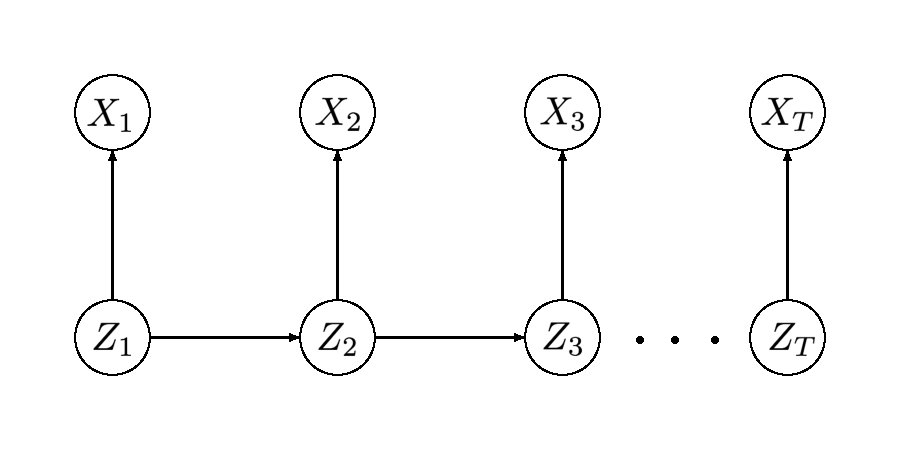
\includegraphics[width=.8\linewidth]{hmm_graph.pdf}
  \caption{{\bf Grahpical Model of HMM}}
  \label{fig:hmm_graph}
\end{figure}

\subsection{Forward-Backward Algorithm}
We here discuss how to compute the smoothed marginal $p(z_t = j| \vec{x})$ and tghe smoothed two-sliced marginal $p(z_{t-1},z_t| \vec{x})$.\footnote{Note that in online setting, we can only compute $p(z_t = j| \vec{x_{1:t}})$, so called filtered marginal, but we concentrate on the offline setting here.}

Taking a look at the graphical model in Fig(), we can see conditioning on $z_t$ eable to decompose joint distribution into two parts: the past and the future. 
\begin{eqnarray}
p(z_t= k| \mathbf{x}) \propto p(z_t=k, \mathbf{x}_{t+1:T}| \mathbf{x}_{1:t})  \propto p(z_t=k|\mathbf{x}_{1:t}) p(\mathbf{x}_{t+1:T}|z_t=k)
\end{eqnarray}
Let us define forward variables $f_{t,k} = p(z_t = k | \vec{x}_{1:t})$, the bilief of the state given all the previous sequence. 
Also, define backward variables $b_{t,k} = p(\mathbf{x}_{t+1:T}|z_t=k)$, the conditional likelihood of future evidence give the hidden staetes $z_t$.
Forward variables are efficiently computed using dynamic programming. The base case and the recursive relationship is given as follows:
\begin{eqnarray}
  f_{t,k} &=& p(z_t = k | \vec{x}_{1:t}) \nonumber \\
          &=& \frac{p(z_t = k, x_t|\vec{x}_{1:t-1})}  {p(x_t|\vec{x}_{1:t-1})} \nonumber \\  
          &=& \frac{p(x_t|z_t=k, \cancel{\vec{x}_{1:t-1}})p(z_t = k|\vec{x}_{1:t-1})}  {p(x_t|\vec{x}_{1:t-1})} \nonumber \\  
          &=& \frac{p(x_t|z_t=k) \sum_{j=1}^K p(z_t = k | z_{t-1} = j)p(z_{t-1} = j|\vec{x}_{1:t-1})}  {p(x_t|\vec{x}_{1:t-1})} \nonumber \\  
          &=& p(x_t| z_t = k) \sum_{j=1}^K  \beta_{j,k} f_{t-1,k} \\
  f_{1, k} &=& p(z_1 = k) = \alpha_k
\end{eqnarray}
\footnote{MEMO: should we define emission notation e.g. $\psi_{t,k}$}
Similarly, backward variables are computed using following equations:
\begin{eqnarray}
b_{t-1,j} &=& p(\vec{x}_{t:T}|z_{t-1}=j) \nonumber \\
          &=& \sum_{j=1}^K p(\vec{x}_{t:T}, z_{t}=j| z_{t-1}=j) \nonumber \\
          &=& \sum_{j=1}^K p(z_{t}=k| z_{t-1}=j) p(\vec{x}_{t:T}| z_t=k, \cancel{z_{t-1}=j}) \nonumber \\
          &=& \sum_{j=1}^K p(z_{t}=k| z_{t-1}=j) p(x_t|z_t=k) p(\vec{x}_{t+1:T}| z_t=k) \nonumber \\
          &=& \sum_{j=1}^K \beta_{j,k} \psi_{t,k} b_{t,k}  
\end{eqnarray}
Now, we can compute smoothed posterior using forward and backward variables. Let us denote smoothed posterior $\gamma_{t,k} = p(z_t = k|\vec{x}_{1:T})$ and smoothed two-sliced marginal $\xi_{t,j,k} = p(z_{t-1},z_t| \vec{x})$

\begin{eqnarray}
  \gamma_{t,k} &\propto& f_{t,k} b_{t,k}
\end{eqnarray}
Also, smoothed two-sliced marginal is computed as follows:
\begin{eqnarray}
  \xi_{t,j,k} 
  &=&  p(z_{t-1},z_t| \vec{x}_{1:T}) \nonumber \\
  &\propto& p(z_t, z_{t-1}, \vec{x}_{t:T}|\vec{x}_{1:t-1}) \nonumber \\
  &=& p(z_{t-1}|\mathbf{x}_{1:t-1})p(z_t, \mathbf{x}_{t:T}|z_{t-1}, \cancel{\mathbf{x}_{1:t-1}}) \nonumber \\
  &=& p(z_{t-1}|\mathbf{x}_{1:t-1})p(z_t|z_{t-1})p(\mathbf{x}_{t:T}|z_t, \cancel{z_{t-1}}) \nonumber \\
  &=& p(z_{t-1}|\mathbf{x}_{1:t-1})p(z_t|z_{t-1})p(x_t|z_t)p(\mathbf{x}_{t+1:T}|z_t, \cancel{x_t}) \nonumber \\
  &=& f_{t-1,j} \beta_{jk} \psi_{tk} b_{t,k}
\end{eqnarray}
\subsection{Parameter Optimizations via EM}
The paramters can be learned from the dataset using EM (Expectation Maximization), which is also called Baum-Welch specifically for HMM. Likelihood function $l(\mathbf{\theta}) = p(\vec{X} | \mathbf{\theta}) = \sum_Z p(\vec{X}, \vec{Z})$ is hard to optimize because it includes partition function over all the possible states of the hidden states. EM, however, can optimize parameters through iterative procedure if the joint distribution over the observed and hidden variables is easy to compute. We first explain EM in general case before moving on EM for HMM.
EM iterate E-step (Expectation step) and M-step (Maximization step) in order. Define the complete data log likelyhoood to be 
\begin{eqnarray}
l_c(\mathbf{\theta}) = \sum_{n=1}^N \ln(\vec{x}^n, \vec{z}^n | \vec{\theta})
\end{eqnarray}
Note that $\vec{z^n}$ is actually not given. We further define auxiliary function $Q(\mathbf{\theta}, \mathbf{\theta}^{old})$
\begin{eqnarray}
Q(\mathbf{\theta}, \mathbf{\theta}^{old}) &=& E_{p(\vec{Z}|\mathcal{D}, \mathbf{\theta}^{old})}[l_c(\mathbf{\theta})] 
\end{eqnarray}
The E-step computes the expectation of complete log likelihood $Q(\mathbf{\theta}, \mathbf{\theta}^{old})$, then the M-step finds $\vec{\theta}$ that maximize the computed expectation.
\begin{eqnarray}
\vec{\theta}^{new} = \argmax_{\vec{\theta}} Q(\mathbf{\theta}, \mathbf{\theta}^{old})
\end{eqnarray}

Now we can apply EM for HMM.
The complete data log likelihood $l_c(\vec{\theta})$ is written down as 
\begin{eqnarray}
l_c(\mathbf{\theta}) = \sum_{n=1}^N \left[ \ln p(z^n_1| \mathbf{\alpha}) 
+ \sum_{t=2}^T\ln p(z^n_t| z^n_{t-1}, \mathbf{\beta})
+ \sum_{t=1}^T\ln p(x^n_t | z^n_{t}, \mathbf{\phi})
\right]
\end{eqnarray}
The auxilary function $Q(\mathbf{\theta}, \mathbf{\theta}^{old})$, the expected complete log likelihood, is given by
\begin{eqnarray}
Q(\mathbf{\theta}, \mathbf{\theta}^{old}) &=& E_{p(\vec{Z}|\vec{x}, \mathbf{\theta}^{old})}[l_c(\mathbf{\theta})] \nonumber \\
&=& \sum_{n=1}^N \left[ \sum_{k=1}^K \gamma^n_{t,k} \ln \alpha_k 
+ \sum_{t=2}^T \sum_{j=1}^K \sum_{k=1}^K \xi^n_{t,j,k}\ln \beta_{j,k}
    + \sum_{t=1}^T \sum_{k=1}^K \gamma^n_{t, k}\ln \psi_{t,k}
\right]
\end{eqnarray}
In the M step, we optimize $Q$ w.r.t. $\mathbf{\theta} = \{ \mathbf{\alpha}, \vec{\beta}, \vec{\phi}\}$. Firstly, let us consider the optimization of $\vec{\alpha}$. Using Lagrange Multiplier with the constraint $\sum_k \alpha_k = 1$, we obtain the optimal $\vec{\alpha}$. 
\begin{eqnarray}
  L_{\vec{\alpha}}(\vec{\theta}, \lambda)
 &=& Q(\mathbf{\theta}, \mathbf{\theta}^{old}) + \lambda (1 - \sum_k \alpha_k) \\ 
  \pard{L_{\vec{\alpha}}(\vec{\theta}, \lambda)}{\alpha_k} &=& \frac{\sum_{n=1}^N \gamma^n_{t,k}}{\alpha_k} - \lambda \\
  \pard{L_{\vec{\alpha}}(\vec{\theta}, \lambda)}{\lambda} &=& (1 - \sum_k \alpha_k) 
\end{eqnarray}
Seeking stationary point, that is $ \pardi{L_{\vec{\alpha}}(\vec{\theta}, \lambda)}{\alpha_k} = \pardi{L_{\vec{\alpha}}(\vec{\theta}, \lambda)}{\lambda} = 0$, we obtain the optimal initial probability $\alpha^*_k$.
\begin{eqnarray}
\alpha^*_k = \frac{\sum_{t=1}^T \gamma^n_{t, k}}{\sum_{t=1}^T \sum_{l=1}^{K}\gamma^n_{t, l}}
\end{eqnarray}
Similary, using appropriate Lagrange Multiplier, we obtain the optimal transition probability $\beta^*_k$.
\begin{eqnarray}
\beta^*_{j,k} = \frac{\sum_{T=2}^T \xi_{t-1, t, j, k}}{\sum_{t=2}^T \sum_{l=1}^{K}\xi_{t-1, t, j, l}}
\end{eqnarray}
Assume the emission probability is categorical distribution
\begin{eqnarray}
p(x_t = m | z_t = k, \vec{\phi}) = \mu_{k, m}
\end{eqnarray}
where $\vec{\phi} = \{\vec{\mu}\}$. $\vec{\mu}$ is $K \times M$ matrix where $M$ is the number of the categories. 
Lagrange function of the emission parameter with corresponding constraint and its partial derrivatives are  given by
\begin{eqnarray}
  L_{\vec{\mu}}(\vec{\theta}, \vec{\lambda}) &=& Q(\mathbf{\theta}, \mathbf{\theta}^{old}) + \sum_{k=1}^{K} \lambda_k (1 - \sum_{m=1}^M \mu_{k, m}) \\
  \pard{L_{\vec{\mu}}(\vec{\theta}, \vec{\lambda})}{\mu_{k,m}} &=& \frac{ N_{k, m} }{\mu_{k, m} }\\
  \pard{L_{\vec{\mu}}(\vec{\theta}, \vec{\lambda})}{\lambda_{k}} &=& 1 - \sum_{m=1}^M \mu_{k, m}
\end{eqnarray}
where $\vec{\lambda} = (\lambda_1, ..., \lambda_K)$ is vector of Lagrange Multipliers. 
$N_{m, k}$ is the weighted counts of output categories given by
\begin{eqnarray}
  N_{k, m} = \sum_{n=1}^N \sum_{t=1}^{T_n} \gamma^n_{t, k} \delta_{x^n_t, m}
\end{eqnarray}
where $\delta_{i,j}$ is Kronecker delta\footnote{should use Iverson bracket? (because we might use simbol for input and hidden states)}.
Now we have the optimal parameter $\mu^*_{k,m}$ by seeking stationary point.
\begin{eqnarray}
  \mu^*_{k,m} = \frac{N_{k,m}}{\sum_{m=1}^{M} N_{k,m}} 
\end{eqnarray}

\subsection{Viterbi decoding}
Choose the optimal sequence of hiden states.
...











%
% Copyright(c) 2015 Taikai Takeda <297.1951@gmail.com> All rights reserved.
%

\def\ba{\bm{a}}
\def\bb{\bm{b}}
\def\bc{\bm{c}}
\def\bd{\bm{d}}
\def\be{\bm{e}}
\def\bg{\bm{g}}
\def\bh{\bm{h}}
\def\bi{\bm{i}}
\def\bj{\bm{j}}
\def\bk{\bm{k}}
\def\bl{\bm{l}}
\def\bn{\bm{n}}
\def\bo{\bm{o}}
\def\bp{\bm{p}}
\def\bq{\bm{q}}
\def\br{\bm{r}}
\def\bs{\bm{s}}
\def\bt{\bm{t}}
\def\bu{\bm{u}}
\def\bv{\bm{v}}
\def\bw{\bm{w}}
\def\bx{\bm{x}}
\def\by{\bm{y}}
\def\bz{\bm{z}}

\def\bA{\bm{A}}
\def\bB{\bm{B}}
\def\bC{\bm{C}}
\def\bD{\bm{D}}
\def\bE{\bm{E}}
\def\bF{\bm{F}}
\def\bG{\bm{G}}
\def\bH{\bm{H}}
\def\bI{\bm{I}}
\def\bJ{\bm{J}}
\def\bK{\bm{K}}
\def\bL{\bm{L}}
\def\bM{\bm{M}}
\def\bN{\bm{N}}
\def\bO{\bm{O}}
\def\bP{\bm{P}}
\def\bQ{\bm{Q}}
\def\bR{\bm{R}}
\def\bS{\bm{S}}
\def\bT{\bm{T}}
\def\bU{\bm{U}}
\def\bV{\bm{V}}
\def\bW{\bm{W}}
\def\bX{\bm{X}}
\def\bY{\bm{Y}}
\def\bZ{\bm{Z}}

\section{Pairwise HMM}
\label{sec:phmm}
Pairwise HMMとは2つのsequence data(DNAの塩基配列やタンパク質のresidue配列)の類似度をモデル化したHMMである.これはdiscrete HMMの拡張であると考えることができるが,一般的なdiscrite HMMとは出力が2つのシンボルの組になるという点で異なる.隠れ状態の状態遷移図は以下のようになる.$M$はMatch状態,$X,Y$はそれぞれの配列の挿入状態を表す.

\begin{figure}[]
  \centering
  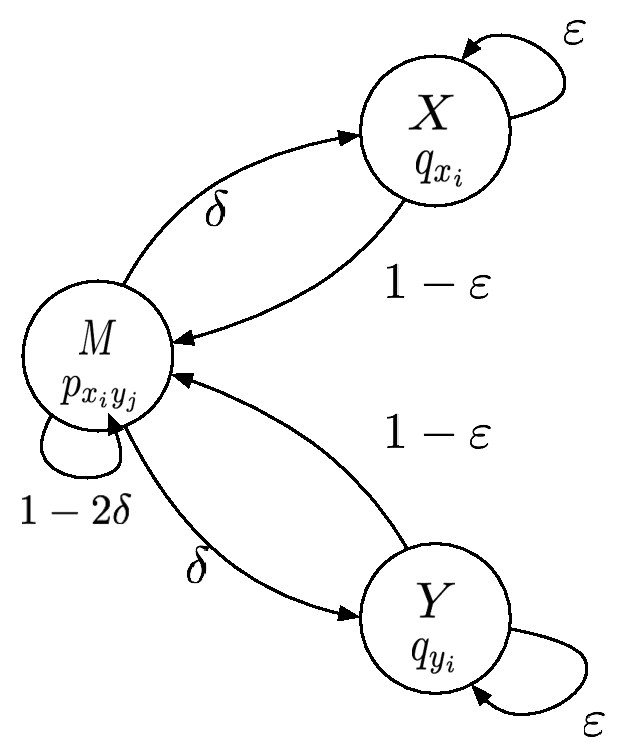
\includegraphics[width=0.3\textwidth, bb=0 0 300 400]{graffe/phmm_simple.pdf}  
  \caption{phmmの状態遷移図}
\end{figure}

\subsection{Notations}
\label{subsec:phmm_nt}
定式化する上でNotationを整理する.観測変数はシンボル列$\bm{x}, \bm{y}$である.
\begin{align}
\bm{x}&=(x^1,...,x^{T_x})\\
\bm{y}&=(y^1,...,y^{T_y})\\
\end{align}
観測変数$x^i, y^j$に対応する隠れ変数$\bm{z}^{ij}$は以下のように定義する.ここで,$x^i$もしくは$y^j$の代わりにgapを許す(観測されたシンボルが対応しない場合がある).
\begin{align}
\bm{z} = 
\begin{pmatrix}
\bm{z}^{11}  & \cdots & \bm{z}^{1 T_y} \\
\vdots  & \ddots & \vdots \\
\bm{z}^{T_x 1}& \cdots & \bm{z}^{T_x T_y}
\end{pmatrix}
\end{align}
隠れ変数は$\bm{z}^{ij}$は状態数$K$に対して1-of-$K$符号化方式で表される.
\begin{align}
\bm{z}^{ij} &= (z^{ij}_1,\ldots,z_K^{ij})\\
z_k^{ij} &= \left\{
\begin{array}{ll}
1 & \mbox{$x^i, y^j$は$k$番目の状態から出力される}\\
0 & \mbox{otherwise}
\end{array}
\right.
\end{align}
また,表記の簡単のため,$\bm{z}^{i0}=\bm{z}^{0j}=0$, 遷移の方向のoffsetとして$\bm{\delta}=\{(\delta_x, \delta_y)\}$と定義する.ここでは,$\bm{\delta}=\{(1,1),(0,1),(1,0)\}$となる.
これを用いて,隠れマルコフモデルの同時分布は以下ように表される.
\begin{align}
  p(\bm{x},\bm{y}, \bm{z}|\bm{\theta})=
p(\bm{z}^{11}|\bm{\alpha})
\prod^{T_x,T_y}_{i,j=1} \prod_{(\delta_x, \delta_y) \in \bm{\delta}}
 p(\bm{z}^{ij}|\bm{z}^{i-\delta_x, j-\delta_y}, \bm{\beta})
% \prod^{T_x,T_y}_{i,j=1}
%   p(\bm{z}^{ij}|\bm{z}^{i-1, j-1}, \bm{\beta})
%   p(\bm{z}^{ij}|\bm{z}^{i-1, j}, \bm{\beta})
%   p(\bm{z}^{ij}|\bm{z}^{i, j-1}, \bm{\beta})
\prod^{T_x,T_y}_{i,j=1}
  p(x^i y^j|\bm{z}^{ij}, \bm{\phi})
\end{align}
上記で,$\bm{\theta}=(\bm{\alpha},\bm{\beta},\bm{\phi})$はHMMのパラメタである.
\begin{align}
\begin{array}{ll}
\mbox{初期確率:}  & p(\bm{z}^{11}|\bm{\alpha})=\prod_{k=1}^K \alpha_k^{z_k^{11}}\\
\mbox{出力確率:}  & p(x^i, y^j|\bm{z}^{ij}, \bm{\phi}) = \prod_{k=1}^K p(x^i, y^j|\bm{\phi}_k)^{z^{ij}_k}\\
\mbox{遷移確率:}  & p(\bm{z}^{ij}|\bm{z}^{i-\delta_x, j-\delta_y}, \bm{\beta}) =  \prod_{l,k=1}^{L,K} \beta_{lk}^{z^{i-\delta_x,j-\delta_y}_l z^{ij}_k}
% & p(\bm{z}^{ij}|\bm{z}^{i-1, j-1}, \bm{\beta}) =  \prod_{k,l=1}^{K,L} \beta_{kl}^{z^{ij}_k z^{i-1,j-1}_l} \\
% &p(\bm{z}^{ij}|\bm{z}^{i, j-1}, \bm{\beta}) =  \prod_{k,l=1}^{K,L} \beta_{kl}^{z^{ij}_k z^{i,j-1}_l}\\
% &p(\bm{z}^{ij}|\bm{z}^{i-1, j}, \bm{\beta}) =  \prod_{k,l=1}^{K,L} \beta_{kl}^{z^{ij}_k z^{i-1,j}_l}
\end{array}
\end{align}
ここで,
\begin{align}
&\bm{\alpha} = (\alpha_1, \ldots, \alpha_K)\in\R^K\label{eq:res_a}\\
&\bm{\beta} =  (\bm{\beta_1}, \ldots ,\bm{\beta}_K)\in\R^K\times\R^K \mbox{ where } \ \bm{\beta}_k=(\beta_{k1},\ldots, \beta_{kK})\in\R^K\label{eq:res_b}\\
&\bm{\phi}  = (\bm{\phi}_1,\ldots,\bm{\phi}_K)
\end{align}
である.

\subsection{Biterbi Algorithm}

\subsection{EM algorithm}

\label{subsec:em}
EM algorithmによりパラメタの最適化を行う.EMアルゴリズムは以下のようなくり返しのアルゴリズムである.
\begin{align}
\mbox{\textbf{E-step}}&\\
&Q(\bm{\theta},\bm{\theta}^{old}) =
  \E_{p(\bm{z}|\bm{x}, \bm{\theta}^{old})}[\ln p(\bm{x}, \bm{z}| \bm{\theta})]\\ \\
\mbox{\textbf{M-step}}&\\
& \ \ \ \ \bm{\theta}^{new} \ \ \  = \argmax_{\bm{\theta}} p(\bm{\theta}, \bm{\theta}^{old})
\end{align}
Estepでは,事後分布$p(\bm{z}^{ij}|\bm{x})$と$p(\bm{z}^{ij}, \bm{z}^{i-\delta_x, j-\delta_y}|\bm{x})$を求める必要がある.
この事後分布はforward-backwardアルゴリズムで効率的に求めることが出来る.forward変数$
f$とbackward変数$b$を以下のように定義する.この2つの変数から,事後分布を求めることが出来る.ここでは,表記の簡単のためパラメタは明記しない.
\begin{align}
f^{ij} &= p(x^{1},\cdots,x^i, y^1,\cdots,y^{j}, \bm{z}^{ij})\\
b^{ij} &= p(x^{i+1},\cdots,x^{T_x}, y^{j+1},\cdots,y^{T_y}| \bm{z}^{ij})\\
\bm{\gamma^{ij}} &= p(\bm{z}^{ij}|\bm{x},\bm{y}) = f^{ij} b^{ij}/p(\bm{x},\bm{y})\\
\gamma^{ij}_k &= p(z^{ij}_k = 1|\bm{x},\bm{y})\\
\bm{\xi^{ij\delta}} &= 
p(\bm{z}^{ij}, \bm{z}^{i-\delta_x, j-\delta_y}|\bm{x},\bm{y}) = 
  f^{i-\delta_x, j-\delta_y} p(\bm{z}^{ij}|\bm{z}^{i-\delta_x, j-\delta_y}) p(x^{ij}|\bm{z}^{ij})b^{ij}  / p(\bm{x},\bm{y})\\
\xi^{ij\delta}_{lk} &= p(z^{ij}_k = 1, z^{i-\delta_x, j-\delta_y}_{l}=1|\bm{x},\bm{y})
\end{align}
ここで,表記の簡単のため$\bm{\gamma},\bm{\xi}$を定義した.すると,これらはDP(Dynamic Programming)で計算できる.
\begin{align}
f^{11} &= p(\bm{z}^{11})p(x^1,y^1|\bm{z}^{11})\\
f^{ij} &=
  p(x^i, x^j|\bm{z}^{ij})
  \sum_{(\delta_x,\delta_y)\in \bm{\delta}}  \sum_{\bm{z}^{i-\delta_x, j-\delta_y}}
  p(\bm{z}^{ij}|\bm{z}^{i-\delta_x, j-\delta_y})f^{i-\delta_x, j-\delta_y}\\
b^{T_xT_y} &= \bm{1} \\
b^{ij} &=
   \sum_{(\delta_x,\delta_y)\in \bm{\delta}}  \sum_{\bm{z}^{i+\delta_x, j+\delta_y}}
         p(x^{i+\delta_x}, x^{j+\delta_y}|\bm{z}^{i+\delta_x, j+\delta_y})
  p(\bm{z}^{i+\delta_x, j+\delta_y}|\bm{z}^{ij})b^{i+\delta_x, j+\delta_y}
\end{align}
Mstepでは,この事後分布$p(\bm{z}|\bm{x},\bm{y},\bm{\theta}^{old})$を用いてQ関数を最大化するパラメタ$\bm{\theta}$を求める.
\begin{align}
Q(\bm{\theta}, \bm{\theta}^{old})&=
\E_{ p(\bm{z}|\bm{x},\bm{y},\bm{\theta}^{old})}
[\ln p(\bm{x},\bm{y},\bm{z}|\bm{\theta})]\\
\bm{\theta}^{new} &= \argmax_{\bm{\theta}} Q(\bm{\theta}, \bm{\theta}^{old})
\end{align}
それぞれのパラメタは以下の通り計算できる.
\begin{align}
  \alpha_k &= \gamma^{11}_k / \sum_k \gamma^{11}_k\\
  \beta_{lk} &= \sum_{ij \bm{\delta}} \xi^{ij\delta}_{lk} / 
               \sum_{ij \bm{\delta}k}b\xi^{ij\delta}_{lk} \\
  \bm{\theta}^*_k &= \argmax_{\bm{\theta}_k} \sum_{ijk} \gamma^{ij}_k p(x_i, y_j|\bm{\theta}_k, z^{ij}_k = 1)
\end{align}
$\bm{\theta}$は,emissionの分布の形$p(x,y|\bm{\theta}, \bm{z})$を仮定することで得ることが出来る.ここでは,シンボルを$s^{1}...s^D$の$D$種類として,$s^m,s^n$の組み合わせを出力する確率を$\mu^{mn}$に持つ多項分布を仮定する.
\begin{align}
p(x,y| \bm{\phi}) = \prod_{mn} \mu_{mn}^{I(x, s^m) I(y, s^n)}
\end{align}
このとき,パラメータ$\bm{\phi} = \bm{\mu}$はラグランジュの未定乗数法を用いて以下のように求められる.
\begin{align}
  \mu^{mn} = \sum_{ij} \gamma^{ij} I(x^i, s^m) I(y^j, s^n)/ \sum_{ijmn} \gamma^{ij} I(x^i, s^m) I(y^j, s^n)
\end{align}
以上を用いて,パラメタの最適化を行うことができる.




\printbibliography
%\input{appendix}
\end{document}
